\section{Solving MDPs}
\label{sec:solve}

\subsection{Ways to solve MDPs}

We categorize MDP solving into

\begin{itemize}
    \item Model-based solutions, which solve MDPs that are model based, i. e., full transition dynamics is known. Hereunder we have to methods
    \begin{itemize}
        \item Value iteration
        \item Policy iteration
    \end{itemize}
    \item Model-free solutions, which solve problems where the transition dynamics are unknown.
    \begin{itemize}
        \item Q-learning
        \item SARSA
    \end{itemize}
\end{itemize}

\subsection{Model-based solutions}

\subsubsection{Value iteration}

Value iteration is a method where the value function is estimated first, and then the policy is computed from the value function. The update rule in \Cref{eq:update_V} is used at each step,

\begin{align}
    V_{t+1} &= \max_a \sum_{s'} T(s, a, s')(R(s, a, s') + \gamma V_t(s')) \\
    &= \max_a Q_{t+1}(s, a)
    \label{eq:update_V}
\end{align}
which is guaranteed to converge in the limit towards $V^*$. After it has converged, the policy is computed. We can also observe that the Q-function is computed at the intermediate steps. Because of the max operator, the system becomes unlinear and has to be solved by iteration, as in this method.

\subsubsection{Policy iteration}

The method of policy iteration finds the value function of the policy for the next timestep and compares this to the action-value function at the next timestep. We do

\begin{itemize}
    \item \textbf{Policy evaluation}: Estimate $V^{\pi}$
    \item \textbf{Policy improvement}: Generate alternative policy $\pi' = \text{argmax}_a Q_{t+1}(s, a) \geq \pi$ as a greedy step.
\end{itemize}

If the improvements stop, then the Bellman optimality equation has been satisfied, and $\pi$ is an optimal policy.

In other words, every timestep, we look one step ahead and think "is it wise to follow the policy I have decided on, or is it better to do a different action? If so, the policy is updated with the better action.

In policy iteration there is no max operator and thus the problem becomes linear and we can solve the system of linear equations to find $V^*(s)$.


\textbf{Generalized Policy Iteration (GPI)} is a term used to describe the concept of letting the policy evaluation and policy improvement processes interact. The policy is improved with respect yo the value function, thus being a locally greedy policy, and the value function is driven towards the value function of the policy. This is the case for almost all reinforcement learning algorithms. See \Cref{fig:gpi} for an illustration.

\begin{figure}[h]
    \centering
        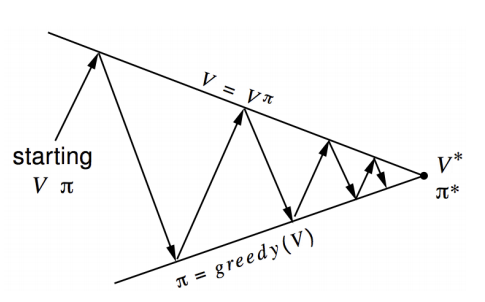
\includegraphics[width=0.8\textwidth]{figures/solving/GPI.PNG}\\
        \caption{The generalized police iteration concept illustrated.}
        \label{fig:gpi}
\end{figure}


\subsubsection{Dynamic programming}

Dynamic programming is often used in model based solvers. Dynamic programming can be used in problems that satisfy the two properties

\begin{itemize}
    \item Optimal substructure: Optimal solution can be decomposed into subproblems
    \item Overlapping subproblems: Subproblems recur many times. Solutions can be cached an reused, as you do in e.g. value iteration, where the temporary value function is stored. 
\end{itemize}

MDPs satisfy both these properties, as the Bellman equations give recursive decomposition, i. e. optimal substructure, and the value function stores and reuses solutions. Again, this is assuming full knowledge of the MDP.

\subsection{Reinforcement learning and MDPS}
Reinforcement learning is a way to solve problems described as MDPs, when
no prior knowledge about the MDP is presented. This means that the agent has to interact and experiment with the environment in order to gain knowledge about how to optimize its behaviour, guided by the rewards as evaluative feedback.

RL adds to MDPs a focus on approximation and incomplete information, and the need for sampling and exploration. The lack of a model generates the need to sample the MDP and gather statistical knowledge about the unknown model.

\subsection{Model Free solutions}

In model free solutions, we categorize the methods in

\begin{itemize}
    \item \textbf{Indirect/model based RL}: Learning the transition and reward model from interaction with the environment. This can be hard to obtain, and the agent has to learn the characteristics of the environment by exploration.
    \item \textbf{Direct/model free RL}: Estimating value functions or policies directly. 
    \item Mixed forms exist as well.
\end{itemize}

\subsubsection{Temporal credit assignment}

Another aspect of the model free solutions is the temporal credit assignment problem, i. e., when to assign rewards to the agent. It can be difficult to assess the utility of some action, if the real effect of it can only be perceived much later. One possibility is to wait until the end of an episode and punish specific actions along the path. Another possibility is to use similar mechanisms as is value iteration to adjust the estimated value of a state based on the immediate rewars and the estimated (discounted) value of the next state. This is generally called \textbf{temporal difference learning}, and it is a general mechanism underlying model-free methods.


\subsubsection{Online RL}

Online RL is the class of RL algorithms that interact with the environment and update their estimates after each experience. Here the concept of \textbf{exploration vs exploitation} is introduced, which is the concept of choosing a different action than the action that is best according to your current estimate.

\subsubsection{Temporal difference learning}

Temporal difference learning algorithms learn estimates of values based on other estimates, which is called bootstrapping. Each step in the world creates a learning example which can be used to bring some value in accordance to the immediate reward and the estimated value of the next state or state-action pair, and we dont have to wait until the end of a trial to make updates along the path.

TD methods do not require a model of the MDP. Another advantage is that the methods are online and incremental, s. t. they can be easily used in various circumstances.

\subsubsection{TD(0)}

TD(0) Does the job of predicting the value of the next step by estimating the value function with the update rule

\begin{align}
    V_{k+1} &:= V_k(s) + \alpha(r + \gamma V_k(s') - V_k(s)) \\
    \label{eq:td0}
\end{align}


The part $\gamma V_k(s') - V_k(s)$ tells the agent how much it improved by going from state $s$ to $s'$. The backup is performed \textit{after} experiencing the transition from state $s$ to $s'$ based on action $a$ and reward given, $r$.


\subsubsection{Q-learning}

The logic behind Q-learning and TD(0) is the same, except that in Q-learning it is the action-value function that is estimated after an experience. The update rule is a variation of the TD learning scheme,

\begin{align}
    Q_{k+1} &:= Q_k(s, a) + \alpha(r + \gamma \max_{a'} Q_k(s', a') - Q_k(s, a)) \\
    \label{eq:qlearn}
\end{align}

The part $\gamma \max_a Q(s_{t+1}, a)$ returns the maximum possible action value in the state we arrive in, and 
$\gamma \max_a Q(s_{t+1}, a) - Q(s_{t}, a_t)$ thus returns a measure of how much better it is to get to the next state, as in TD(0).

Note that, for both TD(0) and Q-learning, the transition function and reqard function is omitted and a measure of how much better it is to move to a new state is being used instead.

Q-learning is called off-policy because the updated policy is different from the behaviour policy, as it estimates the reward for future actions and appends the value to the new state without actually following a greedy policy. In Q-learning, the agent follows some exploration policy based on Q and an exploration strategy, instead of following the estimated optimal policy directly.

The algorithm is exploration insensitive and will converge to the optimal policy regardless of exploration policy, given that a state-action pair can be visited infinite times and $\alpha$ is decreased properly.

\subsubsection{SARSA}

The SARSA method is a lot like Q-learning, but without the maximum in the update step.

\begin{align}
    Q_{k+1} &:= Q_k(s, a) + \alpha(r + \gamma Q_k(s', a') - Q_k(s, a)) \\
    \label{eq:qlearn}
\end{align}

Instead of the max function to find the best estimated action, the action is chosen directly from an $\epsilon$-greedy policy. Hence, its an \textbf{on-policy} algorithm.

\textbf{Difference between Q-learning and SARSA}:
\begin{itemize}
    \item In both cases the action chosen is chosen from an $\epsilon$-greedy policy.
    \item They differ in the way Q is updated after the action, as SARSA still uses the $\epsilon$-greedy policy here, while Q-learning uses a greedy policy with the max-operator. 
    \item Q-learning is more aggressive and will take shortest paths because they are optimal, while SARSA will take longer, safer routes to avoid unexpected negative rewards. Thus, if mistakes are costly, SARSA should be chosen over Q-learning.
\end{itemize}

\begin{figure}[h]
    \centering
        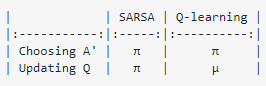
\includegraphics[width=0.5\textwidth]{figures/solving/sarsa_q.PNG}\\
        \caption{Difference between Q-learning and SARSA. $\pi$ is the $\epsilon$-greedy policy, while $\mu$ is a greedy policy.}
\end{figure}